The design approach described in this article is not intended to
replace sound engineering of an intelligent system, but rather as 
an additional step that may be applied in order to provide
the system with more agility, flexibility, and the ability to be rapidly
re-tasked. This is accomplished by assuring that the appropriate knowledge
of the correct scope and format is available to all modules of the
intelligent system.

\begin{figure}[ht!]
\begin{center}
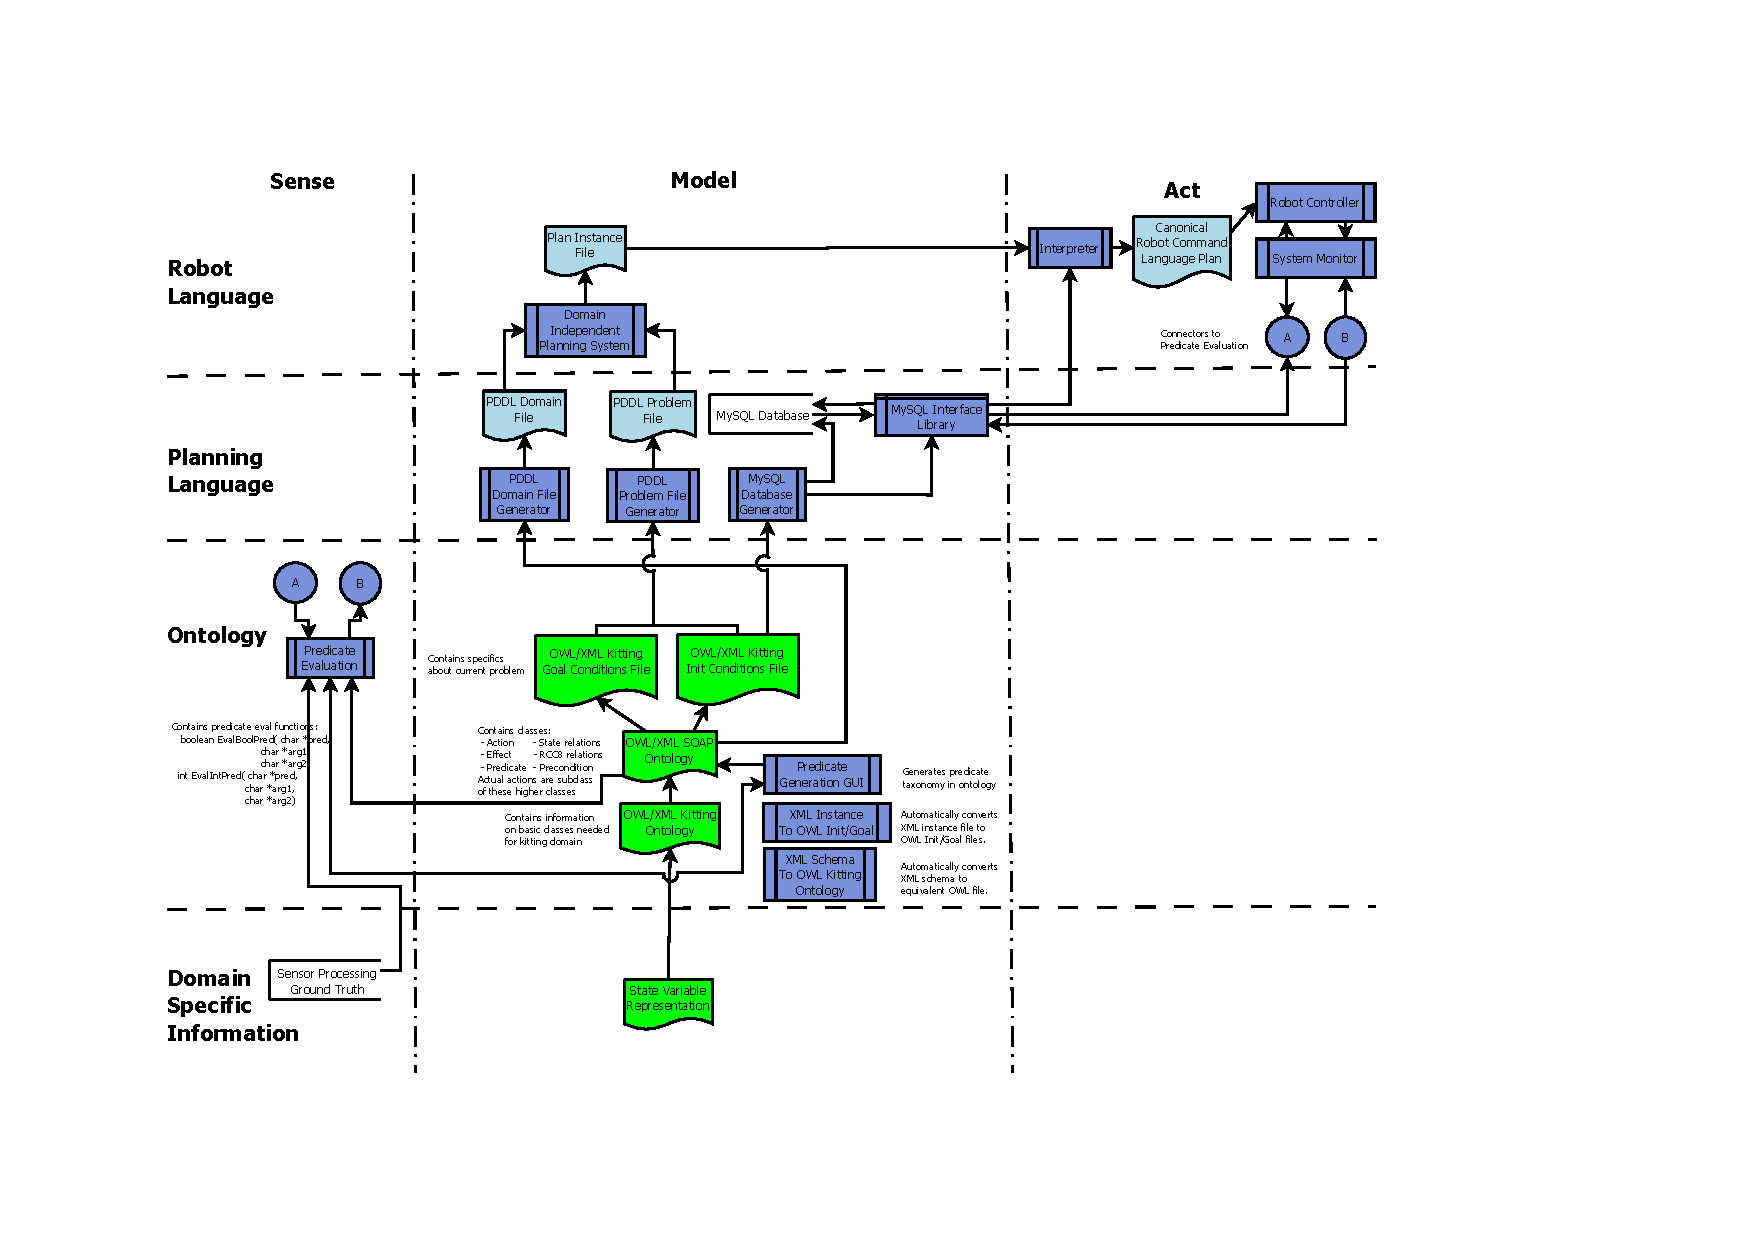
\includegraphics[width=18cm]{images/KnowledgeDrivenRobotics.pdf}
\caption{Knowledge Driven Design extensions- In this figure, green shaded boxes with curved bottoms 
represent hand generated files while
light blue shaded boxes with curved bottoms represent automatically created boxes. Square
boxes represent processes and libraries.}
\label{fig:DesignArchitecture}
\end{center}
\end{figure}

The overall knowledge model of the system may be seen in Figure \ref{fig:DesignArchitecture}.
The figure is organized vertically by the representation that is used for the knowledge
and horizontally by the classical sense-model-act paradigm of intelligent systems.
On the vertical axis, knowledge begins with Domain Specific Information that captures
operational knowledge that is necessary to be successful in the particular domain in which
the system is designed to operate. This information is then organized into a domain
independent representation (an Ontology) that allows for the encoding of an object 
taxonomy, object-to-object
relationships, and aspects of actions, preconditions, and effects. 
Aspects of this
knowledge are automatically extracted and encoded in a form that is optimized for
a planning system to utilize (the Planning Language). Once a plan has been formulated, 
the knowledge is transformed into a representation that is optimized for use by a robotic system
(the Robot Language).

It is acknowledged that sensing and action are important parts of a robotic system.
However, this article focuses on knowledge representation, and thus the modeling section
will be described in the most detail. 

\subsection{Domain Specific Information}
The most basic knowledge that must be gathered for a knowledge
driven system is domain specific information (DSI). This appears along the bottom row of
Figure \ref{fig:DesignArchitecture}. DSI includes sensors and sensor processing that
are specifically tuned to operate in the target domain. Examples of sensor processing
may include pose determination and object identification.

For the knowledge model, a scenario driven approach is taken where
the DSI design begins with a domain expert creating one or more use cases and specific
scenarios that describe the typical operation of the system. Based on these scenarios and 
use cases, the high-level
actions that the system must be able to accomplish can be enumerated and described. 
An action description that includes any preconditions that
must be true for an action to be valid as well as expected effects that will result from a
given action is then created for each action. 

\begin{figure}[ht!]
\begin{center}
\textsl{put-kittray}($\mathit{robot}$,$\mathit{kittray}$,$\mathit{worktable}$): The \textit{Robot} 
$\mathit{robot}$ puts the \textit{KitTray} $\mathit{kittray}$ on the \textit{WorkTable} $\mathit{worktable}$.

\begin{tabular}{ l|l }
  \textit{preconditions} & \textit{effects} \\
  \hline
  \small {\textsf{kittray-location-robot}}(\small $\mathit{kittray}$,\small $\mathit{robot}$)
  &$\neg$\small {\textsf{kittray-location-robot}}(\small $\mathit{kittray}$,\small $\mathit{robot}$)\\
  \small {\textsf{robot-holds-kittray}}(\small $\mathit{robot}$,\small $\mathit{kittray}$)
  &$\neg$\small {\textsf{robot-holds-kittray}}(\small $\mathit{robot}$,\small $\mathit{kittray}$)\\
  \small {\textsf{worktable-empty}}(\small $\mathit{worktable}$)
  &$\neg$\small {\textsf{worktable-empty}}(\small $\mathit{worktable}$)\\
  &\small {\textsf{kittray-location-worktable}}(\small $\mathit{kittray}$,\small $\mathit{worktable}$)\\
  &\small {\textsf{robot-empty}}(\small $\mathit{robot}$)\\
  &\small {\textsf{on-worktable-kittray}}(\small $\mathit{worktable}$,\small $\mathit{kittray}$)\\
\end{tabular}
\caption{Example action along with its preconditions and expected effects.}
\label{fig:ActionExample}
\end{center}
\end{figure}

Based on the action description, objects in the environment that are relevant 
for system operation can be identified. For example, the action depicted in Figure \ref{fig:ActionExample}
has a given robot place a kit tray onto a work table. The preconditions for this action are that
the robot is holding a kit tray and there is a clear space on the table to place the tray. This is
represented by the predicate expressions shown in Figure \ref{fig:ActionExample} that specify that
the robot is holding the kit tray, the kit tray is located on the robot (actually in its gripper), and
the work table is empty. The expected effects of this action are that the kit tray is now located
on the work table and the robot is no longer holding it. This is also represented by a series
of predicates that are shown in Figure \ref{fig:ActionExample}. Based on the preconditions and expected effects,
the objects that are relevant to this action include the robot, the kit tray, and the work table.
Aspects of these items may now be represented in the DSI. For example, that a kit tray has a location and may
be held by the robot or placed on the work table.

\subsection{Ontology}
The design transitions from domain expertise to knowledge modeling expertise
when the SVR is used to generate an ontology which consists of three parts:
\begin{enumerate}
 \item A base ontology that describes the objects in the scenario. This file contains
all of the basic information that was determined to be needed during the evaluation of
the use cases and scenarios. The knowledge is represented in as compact of a form as
possible with knowledge classes inheriting common attributes from parent classes. 
For example, the class for a work table, {\bf WorkTable} is derived from
{\bf BoxyObject}, and {\bf BoxyObject} is derived from {\bf SolidObject}. The actual size of the work table
is defined in the {\bf BoxyObject}. The reason for the extension from {\bf BoxyObject}
The work table itself is part of work station.

 \item Extensions that describe the States of the world and relationships between states,
 Ordering constructs, Actions, and Predicates (the SOAP ontology) 
 that are relevant to the scenario.
 \item Instance files that describe the initial and goal states for the system.
\end{enumerate}
The ontology files are
described in more detail in Section \ref{Sect:Ontology}.

\subsection{Planning Language}

\subsection{Robot Language}
From this point forward, automatic planning tools have been designed to transition 
the knowledge into a planning framework and finally a robot specific framework.

As such, it is assumed that a system has been implemented
that is capable of basic robotic actions. In our case, our knowledge
driven system bottoms out in a Robot Operating System (ROS) control layer
\footnote{Certain commercial/open source software and tools are identified 
in this paper in order to explain our research. Such identification does not imply
recommendation or endorsement by the authors or NIST, nor does it 
imply that the software tools identified are necessarily the best available for the purpose.}.